\documentclass[a4paper,11pt]{scrartcl}
\usepackage[a4paper, left=2cm, right=2cm, top=2cm,bottom=2cm]{geometry}
\usepackage{graphicx}
\graphicspath{ {./Downloads/} }

\title{Project Initiation: Dotted Chart Visualizer for Process Mining}
\author{Elisabeth Buttkus, Ariane Chu, Samir Majeri, Pieter Patonedi, Victor Férnandez }
\begin{document}

\maketitle

\section*{Overview}
\subsection*{Assignment Overview}
Process mining is an important practice in the fields of data science and business process management. The goal is to identify process activities in a process-driven system. The results can be used to solve problems or optimize performance of such systems and is therefore highly valued in companies and institutions. The process information needed for this task is extracted from event logs.

To communicate results of process mining tasks clearly, quality data visualization is key. This is why we chose to implement the dotted chart visualizer which enables us to plot process activities over time and highlight them with a wide range of colors. As a result, it will be quicker to spot differences and identify elements to reach a solid and accurate conclusion.

We aim to develop this visualization tool as a Python based, interactive Django app. Our approach will be based on the dotted chart visualizer that is available in the Java-based ProM framework \footnote{https://promtools.org/doku.php}.

\subsection*{Background}
Using the SVN Repository of the ProM dotted chart visualizer as a reference, we will code a visualizer with equal functionality. This requires from us to fully understand the programming of such a visualizer, based on the Java code of the model ProM tool, and be able to recreate the functionality in the paradigm of the Python language.   


\section*{Business Use Case}
\subsection*{Scope of our assignment}
There is a wide variety of choices when it comes to visualization of data. However, with limited time and resources, we chose to restrict the scope of this project to the implementation of the dotted chart visualizer. This tool enables us the monitoring of process activity over time which is an elementary task in the field of Process Mining and therefore of top priority. Our visualizer will provide a legend chart with important process information and use different colors to make process activities visible. The resulting tool will be of high value for the study of Process Mining.

\subsection*{Key Benefits}
Our finished tool will allow the import of event logs in both the CSV and XES file format which are the most important formats in which event data is available. 
The traces are then displayed as a dotted chart that features a legend for easy readability. The user will be able to modify some of the attributes and adjust the visualization properties according to individual requirements. Each visualization can be downloaded and saved. 
Our dotted chart visualizer is highly accessible as interactions with the app surface are intuitive and easy to understand.

\section*{Feasibility Study}
\subsection*{Theoretical View}
Information systems are becoming more and more intertwined with the operational processes which they support. 
Every event is being recorded by today's information systems. We call a set of such events a ¨Event Log". 
Despite all this effort, organizations are having problems extracting value from these data. 
The goal of process mining is to use event data to extract process-related information, e.g., Dotted charts.
Dotted charts are  an important visualization tool used to represent the information extracted from the event data.
The data may come from different sources like a database system, transaction log or a CSV file. Therefore, it is relevant for 
organizations and businesses to have a suitable tool to enable the visualization of this data based on different formats.

Another way to characterize process mining is with the help of process models which are discovered starting from event data.
One of these models is the Petri nets. Petri nets are the oldest and best investigated process model. They are simple and
many analysis techniques can be applied to them.
In order to enhance these Petri nets, Play in, Play out techniques will be used.

\subsection*{Technical View}

Python 3.8 is going to be the main programming language for this project. Our implementation will take the Java-based dotted chart visualizer of the ProM framework as a reference. 
To handle Process Mining tasks, the Python library PM4Py 2.2.4 will be used. 
To build the app desing and the client/server interaction, Django 3.2 was chosen as a framework. 
The visualization of data will be achieved by use of the Python Pandas 1.2.4 library.

\subsection*{Risks and Mitigation Strategies}

\begin{tabular}{ |p{6cm}|p{1.5cm}|p{8cm}|  }
 \hline
 \multicolumn{3}{|c|}{Risks and mitigation strategies} \\
 \hline
 Risk & Severity & Mitigation strategy \\
 \hline
 Members leaving the team & Low & Asking beforehand if everyone is committed to the course and to the project. When someone wants to leave, we will assign and divide the tasks fairly among the remaining members.\\
  \hline
 Limited knowledge about Process Discovery or Process Mining &   Medium  & Sharing resources among team members and educating each other about the topic. \\
  \hline
 Tension between team members &Low & Encourage dialogue and open communication.\\
  \hline
 Programming problems (specifically concerning python or in general) & High & Communicating problems early on with the team. Other team-members, more fluid in python, can probably help.\\
 \hline
\end{tabular}

\section*{Project Plan}
\subsection*{Gantt Chart}

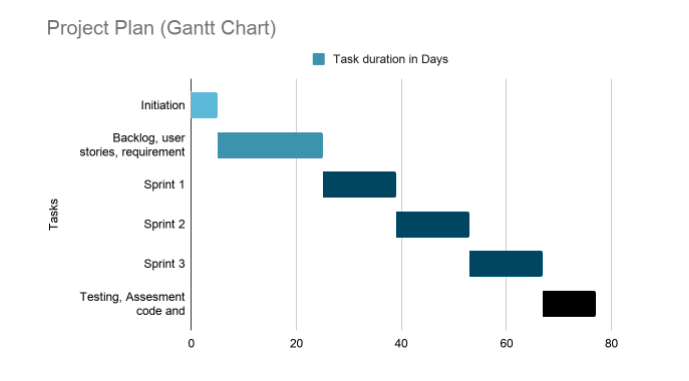
\includegraphics{Gantt}

\section*{Project Team}
\subsection*{Team Member Details}

\vspace{4mm}

\begin{tabular}{ |p{3.2cm}|p{13cm}| }
 \hline
 \multicolumn{2}{|c|}{Team members} \\
 \hline
 Team member & Skillset  \\
 \hline
 Buttkus, Elisabeth   & Prior experience in Python and Java, basic understanding of Process discovery, excellent time management and organization skills (in group environments and individually).     \\
 \hline
 Chu, Ariane & Prior programming experience mainly in Java, basic knowledge of Python, basic understanding of process mining and data mining. Good organizational and communicative skills, very good time management. \\
 \hline
 Majeri, Samir & Prior programming knowledge in Python, Pandas and Django. Successfully finished the lectures and exams of Software Engineering and Web Technologies among others. \\
 \hline
 Patonedi, Pieter  &Bachelor student with prior experience in Java and Python, has a basic knowledge of process mining. Also has experience with unit testing in Python. \\
 \hline
 Robles Fernández, Victor & Bachelor student in computer science with prior experience in Python and its libraries (machine learning, more specific deep learning).Attended the  Business process intelligence (BPI) course.\\
 \hline
\end{tabular}
\\
\vspace{4mm}
\\
\begin{tabular}{ |p{9cm}|p{4.5cm}|p{2cm}|  }
 \hline
 \multicolumn{3}{|c|}{Responsibility at each phase} \\
 \hline
 Phase & Responsible person & Deadline \\
 \hline
 Project initiation and set up infrastructure & Buttkus, Elisabeth    & 19.04.2021\\
 \hline
 Project backlog, user stories, and requirement analysis &   Chu, Ariane  & 09.05.2021\\
 \hline
 Sprint 1 - code and documentation & Patonedi, Pieter
 & 23.05.2021\\
 \hline
 Sprint 2 - code and documentation & Robles Fernández, Victor 
 & 06.06.2021\\
 \hline
 Sprint 3 - code and documentation&  Majeri, Samir
  & 20.06.2021\\
  \hline
 Testing and Assessment code and documentation & Buttkus, Elisabeth  & 30.06.2021\\
 \hline
\end{tabular}

\end{document}
